\subsection{Data}

\subsubsection{Input/Output}

TorchIO uses the medical imaging libraries NiBabel and SimpleITK to read and write images.
Dependency on both is necessary to ensure broad support of image formats.
For instance, NiBabel does not support reading \ac{PNG} files, while SimpleITK does not support some neuroimaging-specific formats.

TorchIO supports up to 4D images, i.e., 2D or 3D single-channel or multi-channel data such as X-rays, \ac{RGB} histological slides, microscopy stacks, multispectral images, \ac{CT}-scans \ac{fMRI} and \ac{dMRI}.


\subsubsection{Data structures}
\label{sec:data_structures}

\paragraph{Image}

The \texttt{Image} class, representing one medical image, stores a 4D tensor, whose voxels encode, e.g., signal intensity or segmentation labels, and the corresponding affine transform, typically a rigid (Euclidean) transform, to convert voxel indices to world coordinates in millimeters.
Arbitrary fields such as acquisition parameters may also be stored.

Subclasses are used to indicate specific types of images, such as \texttt{ScalarImage} and \texttt{LabelMap}, which are used to store, e.g., \ac{CT} scans and segmentations, respectively.

An instance of \texttt{Image} can be created using a filepath, a PyTorch tensor, or a NumPy array.
This class uses lazy loading, i.e., the data is not loaded from disk at instantiation time.
Instead, the data is only loaded when needed for an operation (e.g., if a transform is applied to the image).

\cref{fig:data_structures} shows two instances of \texttt{Image}.
The instance of \texttt{ScalarImage} contains a 4D tensor representing a \ac{dMRI}, which contains four 3D volumes (one per gradient direction), and the associated affine matrix.
Additionally, it stores the strength and direction for each of the four gradients.
The instance of \texttt{LabelMap} contains a brain parcellation of the same subject, the associated affine matrix, and the name and color of each brain structure.

\begin{figure}
  \centering
  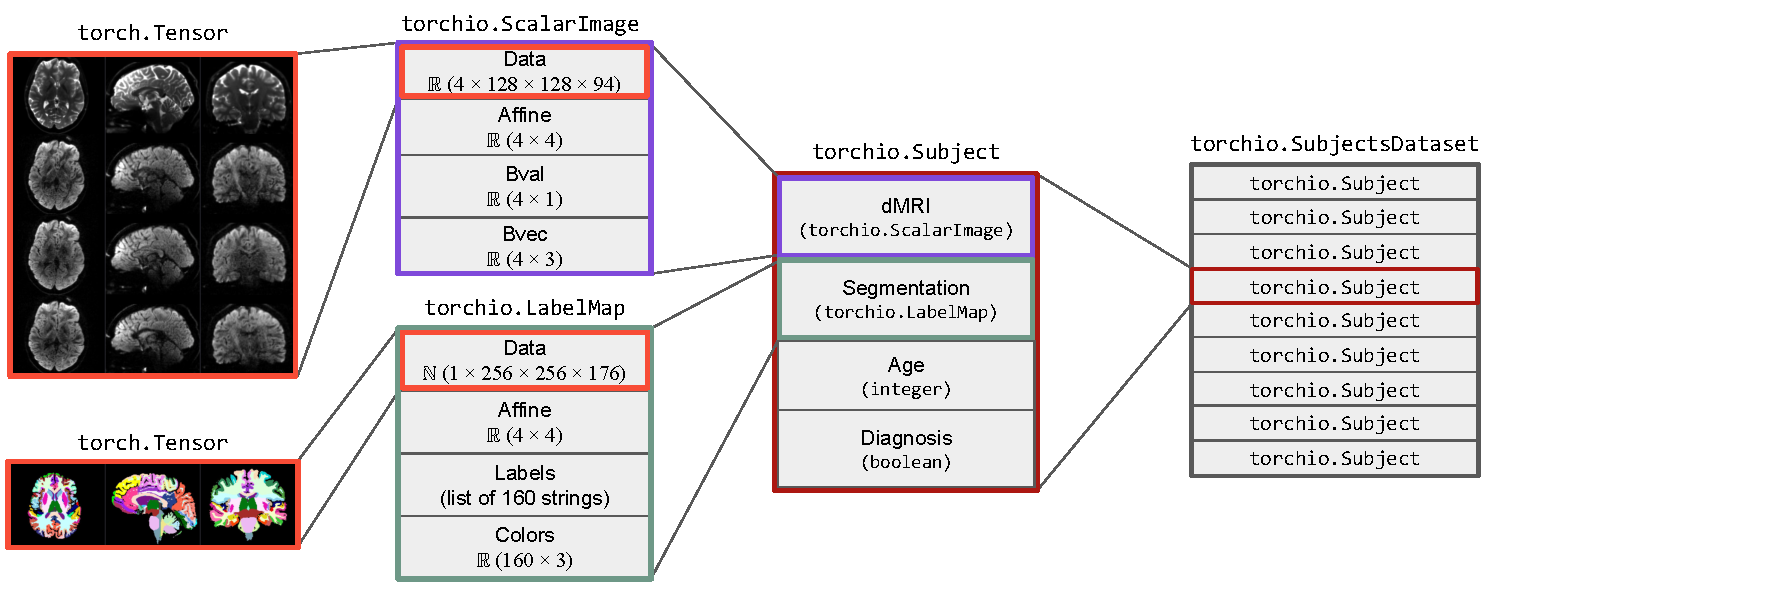
\includegraphics[%
    width=\linewidth,
    trim = {0 0 4.8cm 0},
    clip,
  ]{data_diagram}
  \caption[Usage example of different data structures in TorchIO]{
    Usage example of \texttt{ScalarImage}, \texttt{LabelMap},
    \texttt{Subject} and \texttt{SubjectsDataset}.
    The images store a 4D \ac{dMRI} and a brain parcellation,
    and other related metadata.
  }
  \label{fig:data_structures}
\end{figure}


\paragraph{Subject}

The \texttt{Subject} class stores instances of \texttt{Image} associated to a subject, e.g., a human or a mouse.
As in the \texttt{Image} class, \texttt{Subject} can store arbitrary fields such as age, diagnosis or ethnicity.


\paragraph{Subjects dataset}

The \texttt{SubjectsDataset} inherits from the PyTorch \texttt{Dataset}.
It contains the list of subjects and optionally a transform to be applied to each subject after loading.
When \texttt{SubjectsDataset} is queried for a specific subject, the corresponding set of images are loaded, a transform is applied to the images and the instance of \texttt{Subject} is returned.

For parallel loading, a PyTorch \texttt{DataLoader} may be used.
This loader spawns multiple processes, each of which contains a shallow copy of the \texttt{SubjectsDataset}.
Each copy is queried for a different subject, therefore loading and transforming is applied to different subjects in parallel on the \ac{CPU} (\cref{fig:diagram_volumes}).

An example of subclassing \texttt{SubjectsDataset} is \texttt{torchio.datasets.IXI}, which may be used to download the \ac{IXI} dataset\fnurl{https://brain-development.org/ixi-dataset/}.


\begin{figure}[ht]
  \centering

  \begin{subfigure}{\textwidth}
    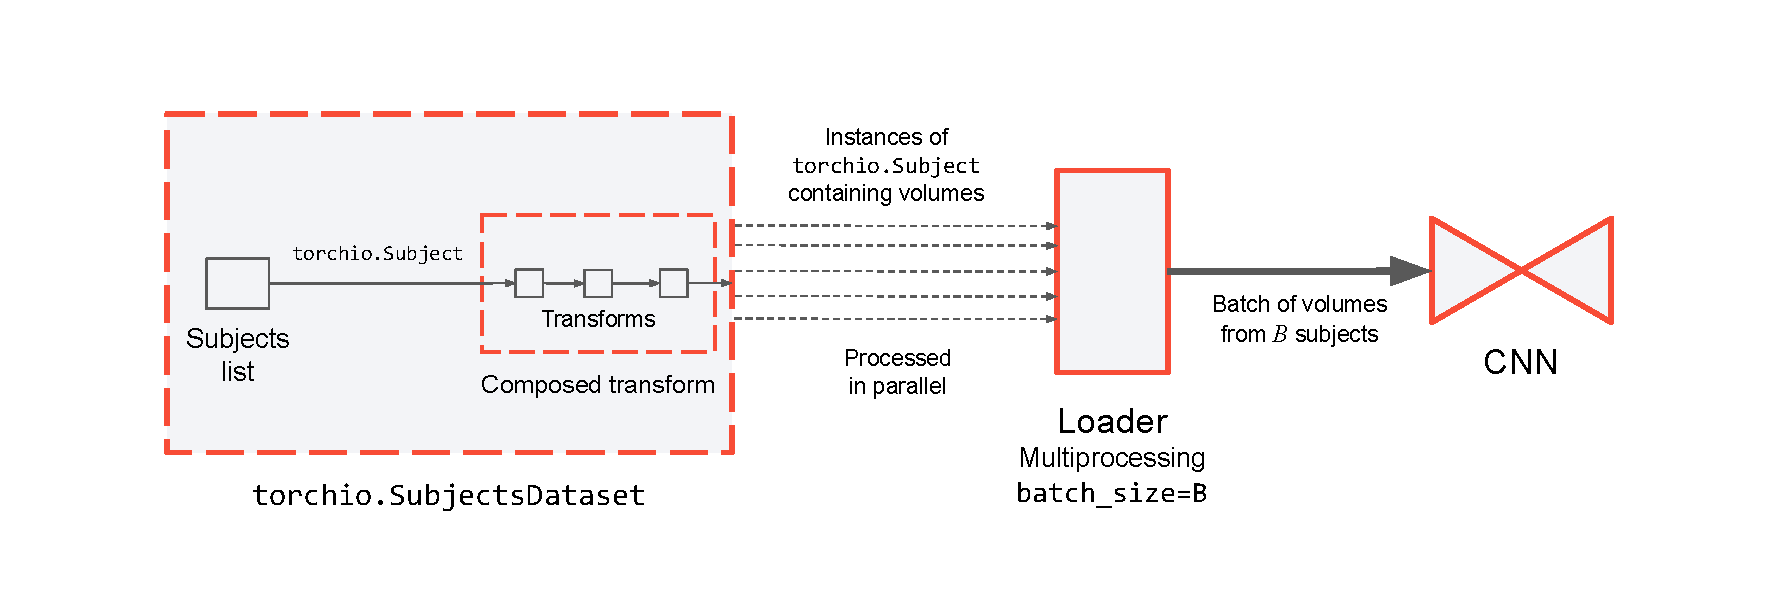
\includegraphics[%
      width=0.98\linewidth,
      trim = {0 1cm 0 1cm},
      clip
    ]
    {diagram_volumes}
    \caption{Training with whole volumes}
    \label{fig:diagram_volumes}
  \end{subfigure}

  \begin{subfigure}{\textwidth}
    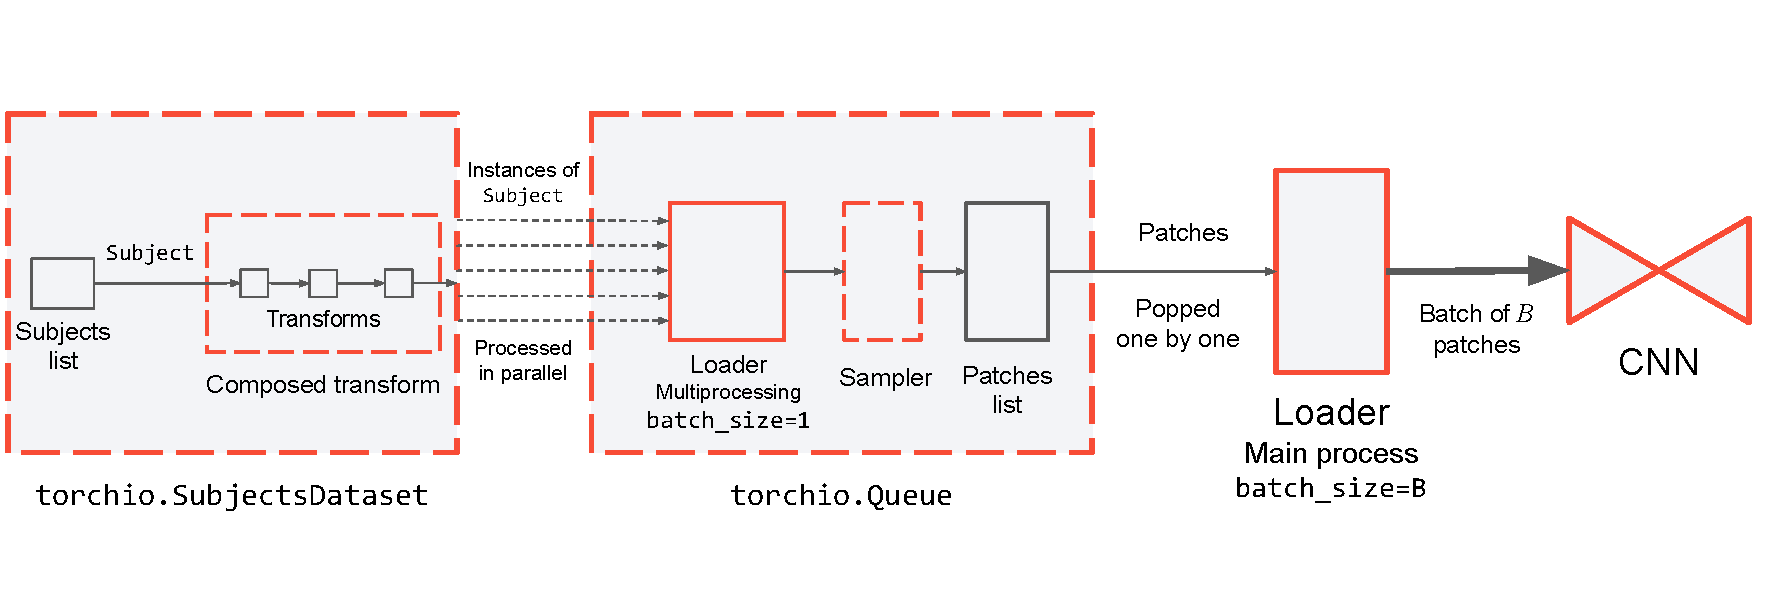
\includegraphics[%
      width=0.98\linewidth,
      trim = {0 0.5cm 0 0},
      clip
    ]
    {diagram_patches}
    \caption{Training with patches}
    \label{fig:diagram_patches}
  \end{subfigure}

  \caption[Data pipelines for training with whole volumes and patches]{
    Diagram of data pipelines for training with whole volumes (top)
    and patches (bottom).
    Boxes with a red border represent PyTorch classes
    (\protect\tikz[baseline=-0.5ex]\protect\draw[thick, color = pytorch_orange] (0,0) -- (0.5,0);)
    or TorchIO classes that inherit from PyTorch classes
    (\protect\tikz[baseline=-0.5ex]\protect\draw[dashed, thick, color = pytorch_orange] (0,0) -- (0.5,0);).
    }
\end{figure}


\subsubsection{Patch-based training}
\label{sec:patches}

Memory limitations often require training and inference steps to be performed using image subvolumes or \textit{patches} instead of the whole volumes, as explained in \cref{sec:computation}.
In this section, we describe how TorchIO implements patch-based training via image sampling and queueing.


\paragraph{Samplers}

A sampler takes as input an instance of \texttt{Subject} and returns a version of it whose images have a reduced \ac{FOV}, i.e., the new images are subvolumes, also called windows or \textit{patches}.
For this, a \texttt{PatchSampler} may be used.

Different criteria may be used to select the center voxel of each output patch.
A \texttt{UniformSampler} selects a voxel as the center at random with all voxels having an equal probability of being selected.
A \texttt{WeightedSampler} selects the patch center according to a probability distribution image defined over all voxels, which is passed as input to the sampler.

At testing time, images are sampled such that a dense inference can be performed on the input volume.
A \texttt{GridSampler} can be used to sample patches such that the center voxel is selected using a set stride.
In this way, sampling over the entire volume is ensured.
The potentially-overlapping inferred patches can be passed to a \texttt{GridAggregator} that builds the resulting volume patch by patch (or batch by batch).


\paragraph{Queue}

A training iteration (i.e., forward and backward pass) performed on a \ac{GPU} is usually faster than loading, preprocessing, augmenting, and cropping a volume on a \ac{CPU}.
Most preprocessing operations could be performed using a \ac{GPU}, but these devices are typically reserved for training the \ac{CNN} so that the batch size and input tensor can be as large as  possible.
Therefore, it is beneficial to prepare (i.e., load, preprocess and augment) the volumes using multiprocessing \ac{CPU} techniques in parallel with the forward-backward passes of a training iteration.

Once a volume is appropriately prepared, it is computationally beneficial to sample multiple patches from a volume rather than having to prepare the same volume each time a patch needs to be extracted.
The sampled patches are then stored in a buffer or \textit{queue} until the next training iteration, at which point they are loaded onto the \ac{GPU} to perform an optimization iteration.
For this, TorchIO provides the \texttt{Queue} class, which inherits from the PyTorch \texttt{Dataset} (\cref{fig:diagram_patches}).
In this queueing system, samplers behave as generators that yield patches from volumes contained in the \texttt{SubjectsDataset}.

The end of a training epoch is defined as the moment after which patches from all subjects have been used for training.
At the beginning of each training epoch, the subjects list in the \texttt{SubjectsDataset} is shuffled, as is typically done in machine learning pipelines to increase variance of training instances during model optimization.A PyTorch loader queries the datasets copied in each subprocess,which load and process the volumes in parallel on the \ac{CPU}.
A PyTorch loader begins by shallow-copying the dataset to each subprocess.
Each worker subprocess loads and applies image transforms to the volumes in parallel.
A patches list is filled with patches extracted by the sampler, and the queue is shuffled once it has reached a specified maximum length so that batches are composed of patches from different subjects.
The internal data loader continues querying the \texttt{SubjectsDataset} using multiprocessing.
The patches list, when emptied, is refilled with new patches.
A second data loader, external to the queue, may be used to collate batches of patches stored in the queue, which are passed to the neural network.
